
\subsection{Allocation Size for Small and Medium Pages}

Since small and medium pages only allow the user to allocate objects in certain size ranges, we can use this to our advantage to store metadata about the allocator in a more efficient way.

Small pages allow objects sizes in the range $S_{small} \in [16B, 256KB]$ and medium pages $S_{medium} \in (256KB, 4MB]$. We note that the allowed sizes in the medium range is an integer multiple of the small range, $S_{medium} = \text{16KB} * S_{small}$. This allows us to limit the allocator to the size range of small page, with an additional multiplication factor of 1 for small pages and 16 KB for medium pages.

With the now limited allocation size range of $S_{small}$ in mind we are able to limit the number of free-lists we need and in turn the bits used in the bitmaps. We need 14 first-levels to be able to index every power of two inside the $S_{small}$ range, with a lower-bound of $2^4 = 16$ and an upper-bound of $2^17 = 256KB$. For efficiency reasons, the number of second levels should be a power of two. Additionally, it would be preferable to be able to store all bitmap information in a single word for performance reasons, both in terms of cache efficiency and bit instructions.

% Additonal benefits are possibility of atomic operations on a 64-bit word.

Combining the insight of the number of required first-levels, second-levels and desire to use a single 64-bit bitmap, we can construct a new bitmap representation. The new bitmap disregards the first-level bitmap all together and combines all second-level bitmaps into a single 64-bit word, where the number of second-levels are 4 ($2^2$). This would give the bitmap representation shown in Figure~\ref{fig:adapted_bitmap}, where there is a single bitmap pointing to the individual free-lists of all possible sizes in $S_{small}$.

\begin{figure}[H]
    \centering
    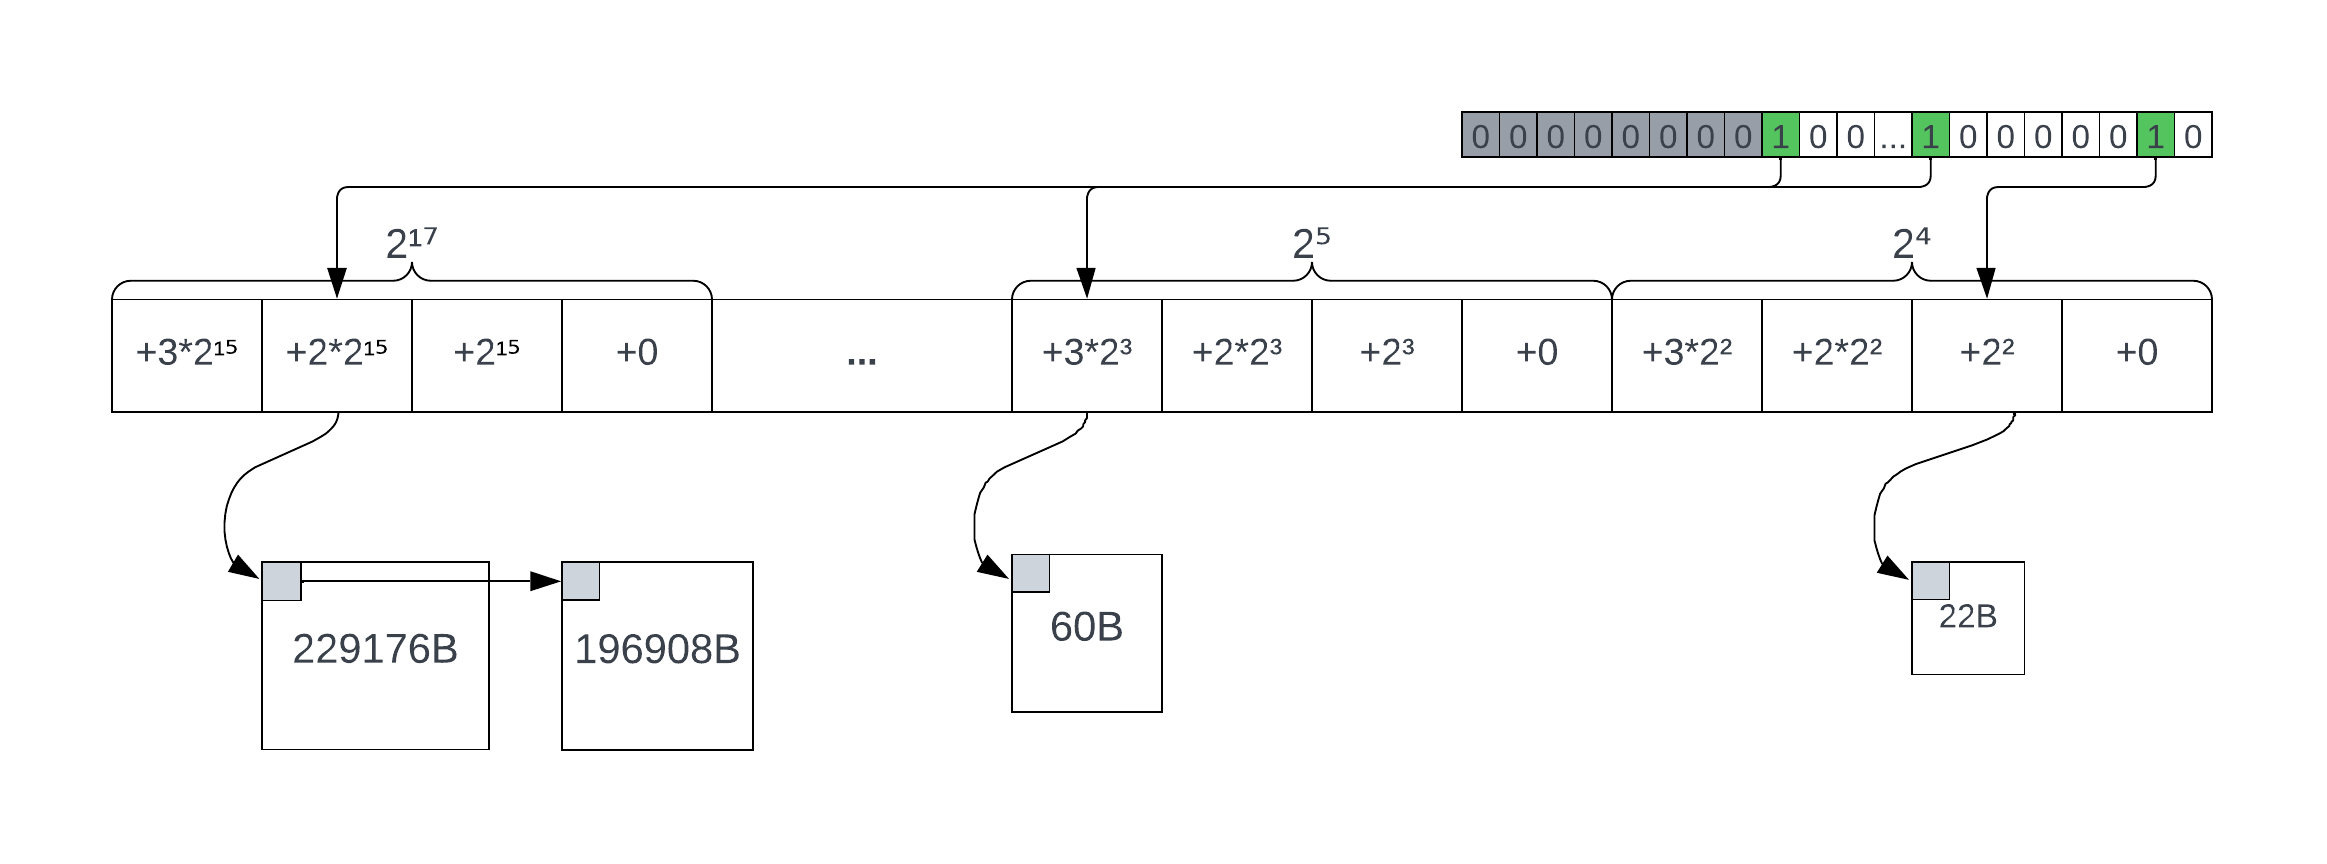
\includegraphics[width=1\textwidth]{figures/adapted_bitmap.png}
    \caption{Adapted 64-bit bitmap representation and how it is used to index free-lists. The most significant 8 bits are unused.}
    \label{fig:adapted_bitmap}
\end{figure}

A major drawback of dividing the memory into only four second-levels per fist-level is that there is less chance that a block is closer to the size that we want to allocate. This could potentially lead to higher fragmentation, as there are fewer size classes of blocks available.

% TODO: Cite TLSF paper.
% Benefits: Reduced memory overhead, cache efficiency, Simplified indexing (and Atomic operations??)
% Drawbacks: Reduce number of second-level partitions to 4, instead of more, which could have an impact on internal fragmentation.

%%% Local Variables:
%%% mode: latex
%%% TeX-master: "main"
%%% End:
